\documentclass[border=10pt]{standalone}

\usepackage{tikz}
\usepackage{tikzsymbols}
\usetikzlibrary{calc,patterns,shapes.geometric}

\def\centerarc[#1](#2)(#3:#4:#5){\draw[#1] ($(#2)+({#5*cos(#3)},{#5*sin(#3)})$) arc (#3:#4:#5);}

\begin{document}
	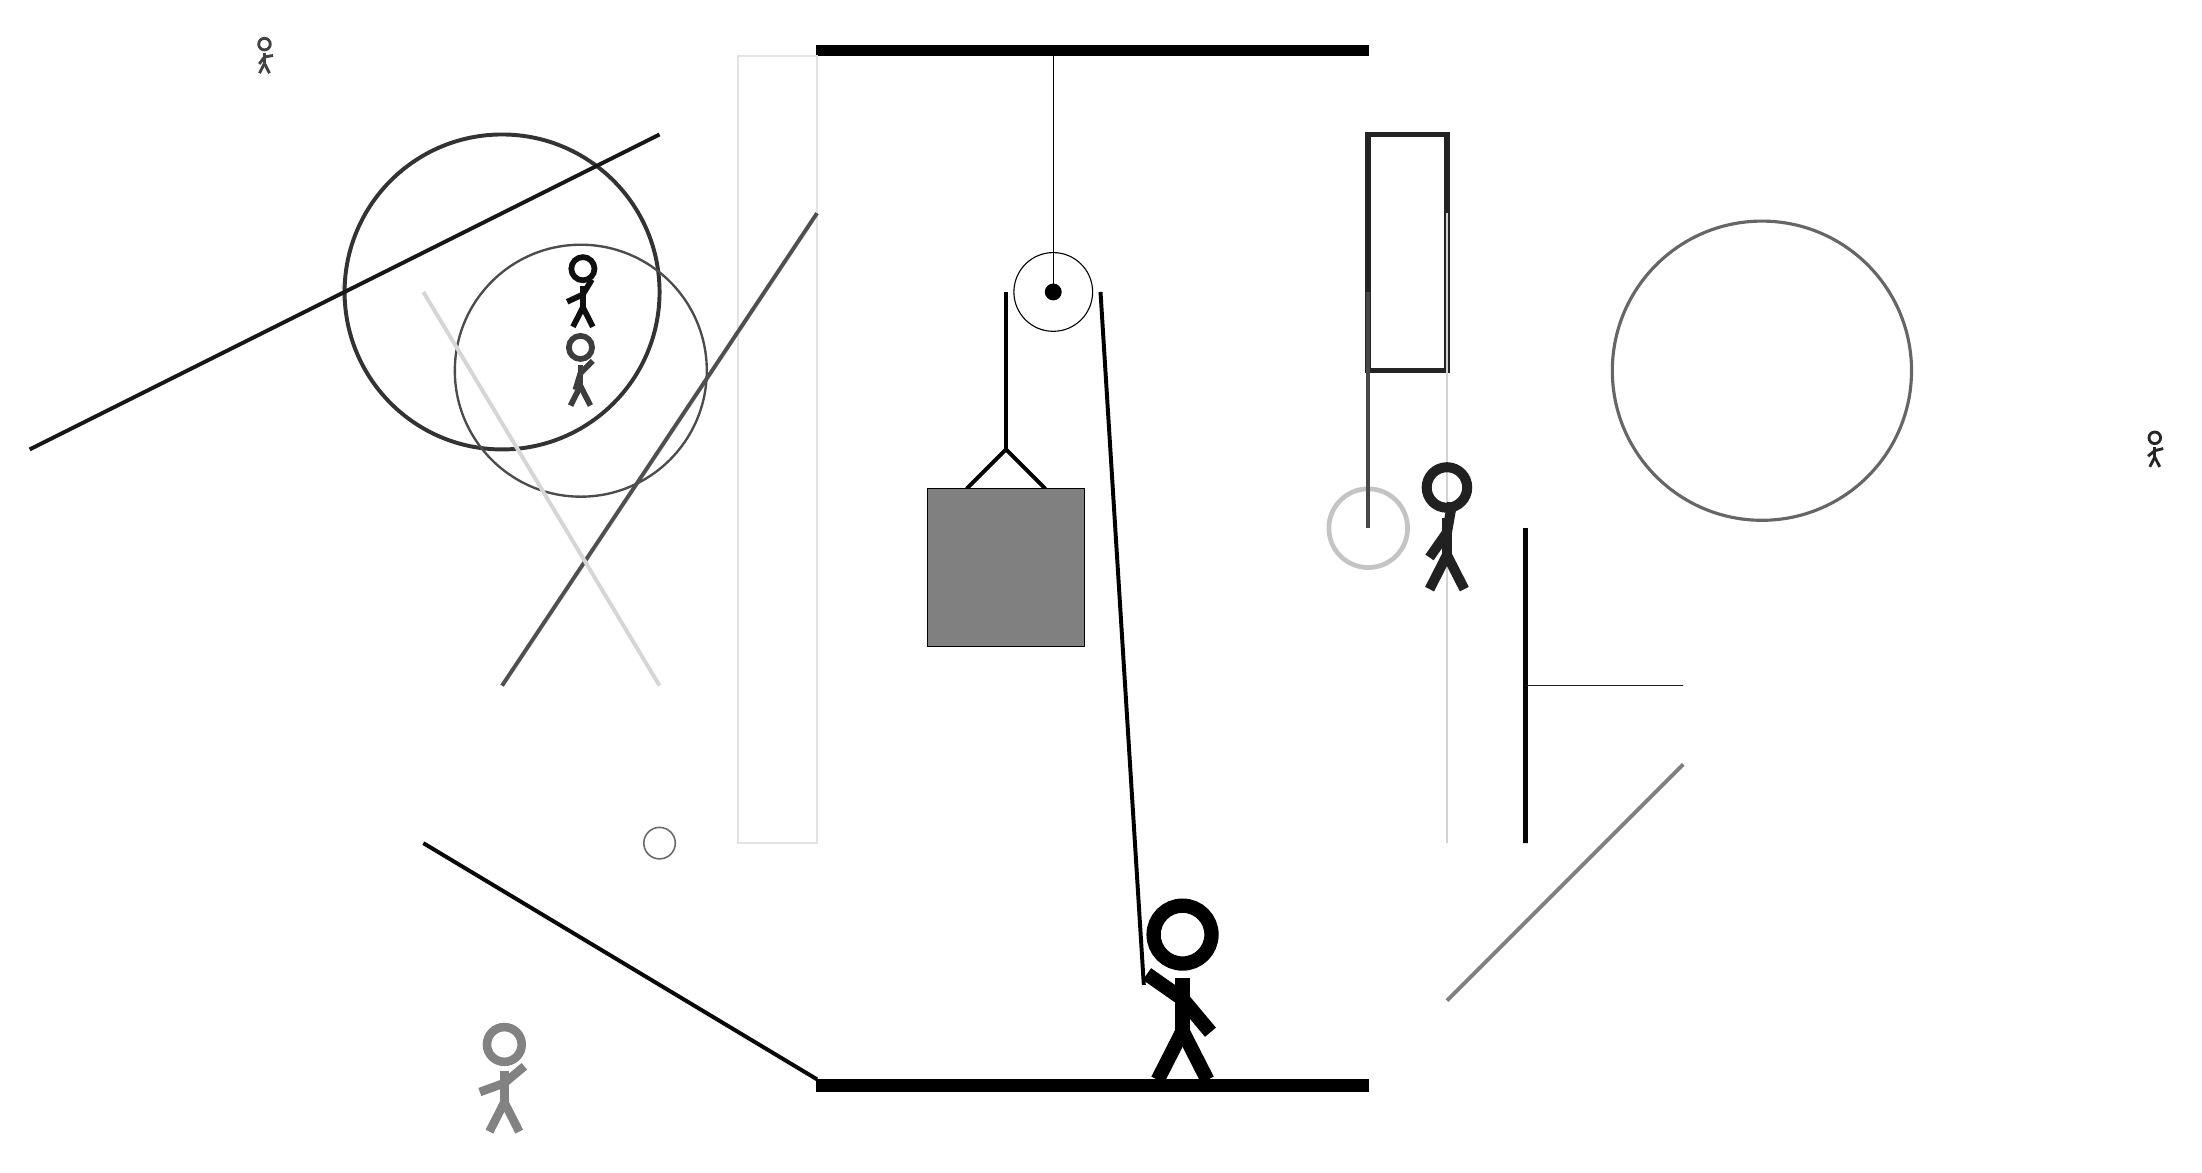
\begin{tikzpicture}
		%%%%% START %%%%%
		
		\draw[fill=black] (-2, 10) rectangle (5, 10.125);
		
		\draw (1, 7) circle (0.5);
		\draw[fill=black] (1, 7) circle (0.1);
		\draw (1, 10) -- (1, 7);
		
		\node[line width=0.2mm, color=black!12] at (-8, 7) {\Strichmaxerl[1][54][17]};
		
		\node[line width=0.5mm, color=black!85] at (15, 5) {\Strichmaxerl[2][39][14]};
		\node[line width=0.4mm, color=black!94] at (-5, 7) {\Strichmaxerl[4][25][59]};
		\node[line width=0.6mm, color=black!74] at (-9, 10) {\Strichmaxerl[2][53][10]};
		\draw [line width=0.6mm, color=black!23](5, 4) circle (0.5);
		
		\draw[line width=0.7mm, color=black!86] (6, 6) rectangle (5, 9);
		
		\draw[line width=0.3mm, color=black!22] (-3, 4) rectangle (-3, 5);
		\draw [line width=0.5mm, color=black!80](-6, 7) circle (2.0);
		\draw[line width=0.5mm, color=black!91](-4, 9) -- (-12, 5);
		\draw [line width=0.2mm, color=black!59](-4, 0) circle (0.2);
		
		\draw [line width=0.3mm, color=black!70](-5, 6) circle (1.6);
		
		\draw[line width=0.3mm, color=black!11] (-3, 0) rectangle (-2, 10);
		\draw[line width=0.5mm, color=black!69](-6, 2) -- (-2, 8);
		\draw[line width=0.5mm, color=black!50](9, 1) -- (6, -2);
		\node[line width=0.4mm, color=black!49] at (-6, -3) {\Strichmaxerl[6][20][40]};
		\draw[line width=0.3mm, color=black!17] (6, 0) rectangle (6, 8);
		
		\draw [line width=0.4mm, color=black!60](10, 6) circle (1.9);
		
		\draw[line width=0.6mm, color=black!98] (7, 0) rectangle (7, 4);
		\node[line width=0.3mm, color=black!76] at (-5, 6) {\Strichmaxerl[4][73][45]};
		
		\node[line width=0.4mm, color=black!87] at (6, 4) {\Strichmaxerl[7][55][80]};
		\draw[line width=0.2mm, color=black!88] (7, 2) rectangle (9, 2);
		
		\draw[line width=0.5mm, color=black!16](-4, 2) -- (-7, 7);
		\draw[line width=0.5mm, color=black!72](5, 4) -- (5, 7);
		\draw[line width=0.5mm, color=black!97](-2, -3) -- (-7, 0);
		
		\draw[line width=0.5mm] (-0.1, 4.5) -- (0.4, 5.0) -- (0.9, 4.5);
		\draw[fill=black!50] (-0.6, 4.5) rectangle (1.4, 2.5);
		
		\draw[line width=0.5mm] (0.4, 7) -- (0.4, 5.0);
		\centerarc[line width=0.5mm](1, 7)(0:180:0.6);
		\draw[line width=0.5mm](1.6, 7) -- (2.15, -1.8);
		
		\node at (2.6, -1.9) {\Strichmaxerl[10][-35][-50]};
		
		\draw[fill=black] (-2, -3) rectangle (5, -3.15);
		
		%%%%% END %%%%%
	\end{tikzpicture}
\end{document}